\section{Frontend}
Das Frontend definiert eine Webpage als Schnittstelle zwischen Anwendern und Dienst, sowie Verwaltungsmöglichkeiten für Administratoren bietet. Zur Navigation bzw Suche von Interfaces und Components werden eine Gesamtliste sowie eine Suchfunktion zur Verfügung gestellt. Es betreibt außerdem eine Datenbank in der alle nötigen Daten gespeichert werden.

\subsection{Use-Cases}

\begin{figure}[!htp]
\begin{center}
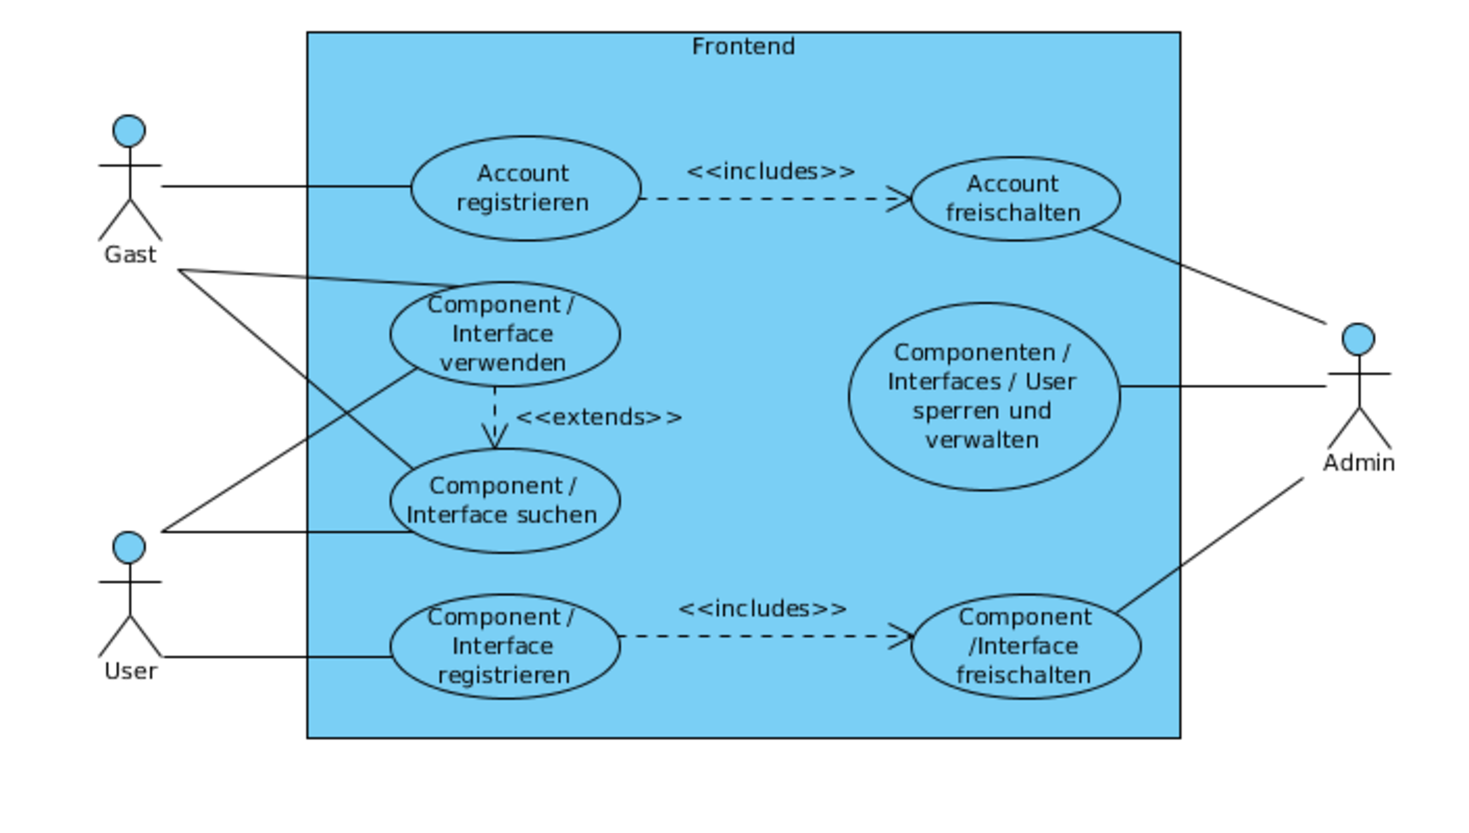
\includegraphics[width=\textwidth]{bilder/use_case_frontend.pdf}
\caption{Use-Case-Diagramm des Frontend}
\label{fig:uc_front}
\end{center}
\end{figure}

Erklärung des Use-Case-Diagramm \ref{fig:uc_front}

1) Ein Gast kann einen Account registrieren. Dieser Account muss daraufhin von einem Admin freigeschaltet werden. Außerdem kann ein Gast eine Component suchen.\\
2) Ein User (mit registriertem Account) kann zusätzlich zum Suchen eine Component auch in sein Programm einbinden und verwenden. Zusätzlich ist es ihm möglich eigenen Components/Interfaces zur Verfügung zu stellen. Bevor diese Components/Interfaces benutzt werden können, müssen sie von einem Admin freigeschaltet werden.\\
3)Zusätzlich zu den bereits angegebenen Funktionen des Freischaltens hat ein Admin die Möglichkeit User/Components/Interfaces zu verwalten bzw. zu sperren.\\